% !Mode:: "TeX:UTF-8:Main"
% arara: pdflatex
% arara: convert: {density: 160, otheroptions: -dispose previous -delay 20 -loop 1, format: gif}
% xarara: showfile: {format: gif}
\documentclass{article}
\usepackage[utf8]{inputenc} %probably not needed ...
\usepackage[T1]{fontenc}
\usepackage{geometry}
\geometry{papersize={128mm,96mm},margin=0.5cm} %\textwidth=11.8, \textheight=8.6
\usepackage[x11names,svgnames]{xcolor}
\usepackage{tikzducks}
\usetikzlibrary{shapes.geometric}
\pagestyle{empty}
\parindent=0pt
\usepackage{animate}
\usepackage{eso-pic}
\usepackage{xfp}
\newcommand\loopmax{10}

\begin{document}
\AddToShipoutPictureBG{%
 \AtPageLowerLeft{%
 %\begin{tikzpicture}[overlay,remember picture]
% %
% \end{tikzpicture}
 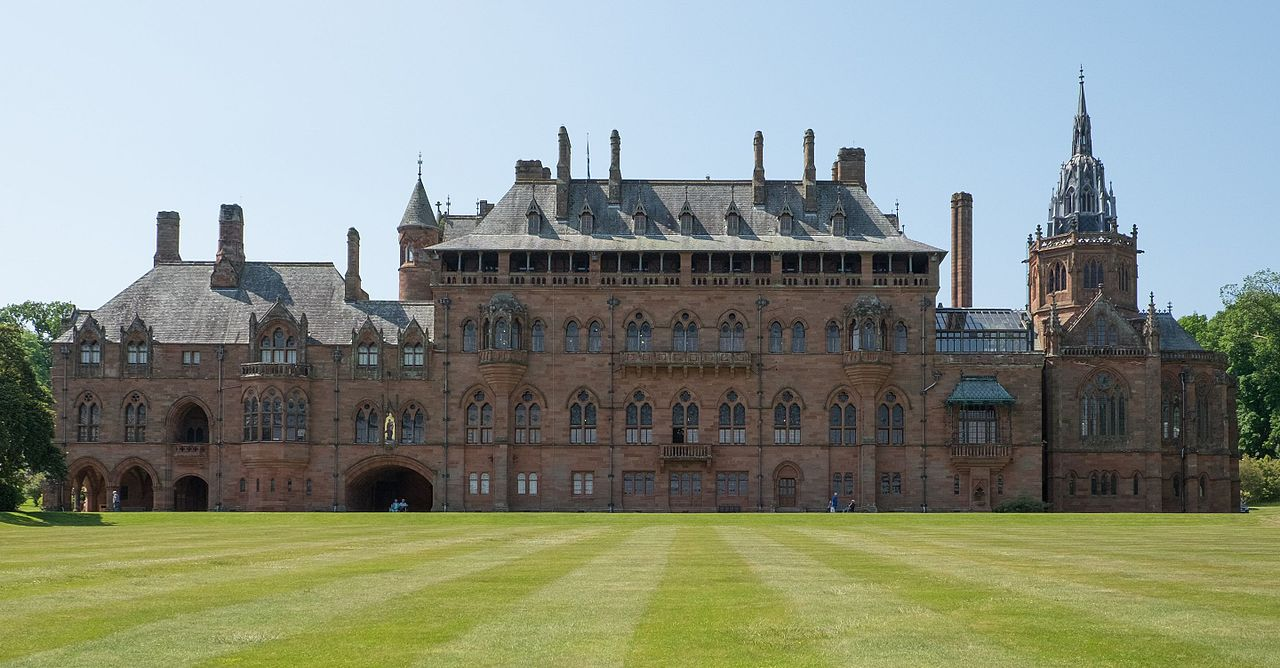
\includegraphics[trim=2cm 0.5cm 0cm 0cm,height=\paperheight]{scotland2-background}%
 }}

\foreach \x in {1,2,...,\loopmax}{%
\begin{tikzpicture}[]
\path[use as bounding box] (0,0) rectangle (\textwidth,\textheight);

% 1. duck
\begin{scope}[xshift=\fpeval{1-\x*(1/\loopmax)}cm,yshift=0.1cm,scale=1.2]

\duck[body=DarkGoldenrod1!20!AntiqueWhite1,beret]
\begin{scope}
\path[clip]
\duckpathjacket;

\node[anchor=south west] at (0,0){
\includegraphics[width=3cm]{tartan3}};
\end{scope}
\draw[thick] \duckpathjacket;

\begin{scope}[rotate=-25]
\draw[line width=1.5pt] (0.13,2.15) ellipse (0.5 and 0.17)
            (0.13,2.25) ellipse (0.55 and 0.17)
	        (0.13,2.4) circle (0.08);
\end{scope}


\begin{scope}[rotate=-25]
\path[clip] (0.13,2.15) ellipse (0.5 and 0.17)
            (0.13,2.25) ellipse (0.55 and 0.17)
	        (0.13,2.4) circle (0.08);
\node[anchor=south west] at (0,1){
\includegraphics[width=3cm]{tartan3}};
\end{scope}

\node[anchor=south west] at (-0.1,-0.55) {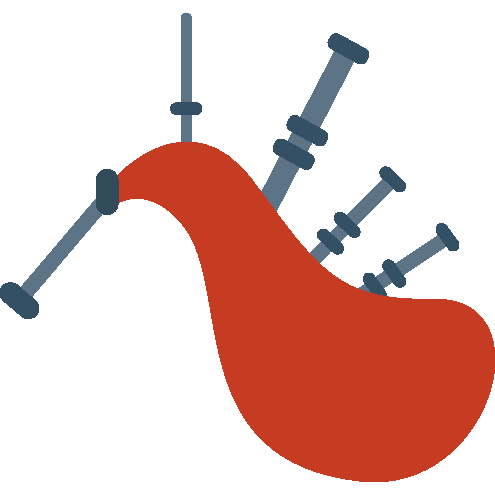
\includegraphics[width=2.1cm]{bagpipes}};
\end{scope}

% 2. duck
\begin{scope}[xshift=\fpeval{5-\x*(1/\loopmax)}cm,yshift=0.1cm,scale=1.2]
\duck[body=DarkGoldenrod1!20!AntiqueWhite1,beret]

\begin{scope}
\path[clip]
\duckpathjacket;

\node[anchor=south west] at (0,0){
\includegraphics[width=3cm]{tartan3}};
\end{scope}
\draw[thick] \duckpathjacket;

\begin{scope}[rotate=-25]
\draw[line width=1.5pt] (0.13,2.15) ellipse (0.5 and 0.17)
            (0.13,2.25) ellipse (0.55 and 0.17)
	        (0.13,2.4) circle (0.08);
\end{scope}

\begin{scope}[rotate=-25]
\path[clip] (0.13,2.15) ellipse (0.5 and 0.17)
            (0.13,2.25) ellipse (0.55 and 0.17)
	        (0.13,2.4) circle (0.08);
\node[anchor=south west] at (0,1){
\includegraphics[width=3cm]{tartan3}};
\end{scope}


\node[anchor=south west] at (-0.1,-0.55) {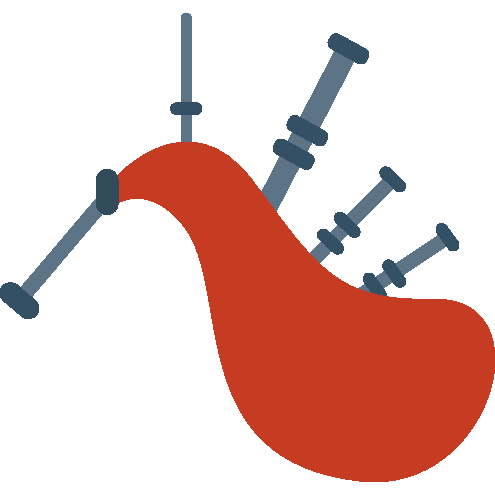
\includegraphics[scale=0.25]{bagpipes}};
\end{scope}

%3. duck
\begin{scope}[xshift=\fpeval{9-\x*(1/\loopmax)}cm,yshift=0.1cm,scale=1.2]
\duck[body=DarkGoldenrod1!20!AntiqueWhite1,beret]

\begin{scope}
\path[clip]
\duckpathjacket;

\node[anchor=south west] at (0,0){
\includegraphics[width=3cm]{tartan3}};
\end{scope}
\draw[thick] \duckpathjacket;

\begin{scope}[rotate=-25]
\draw[line width=1.5pt] (0.13,2.15) ellipse (0.5 and 0.17)
            (0.13,2.25) ellipse (0.55 and 0.17)
	        (0.13,2.4) circle (0.08);
\end{scope}


\begin{scope}[rotate=-25]
\path[clip] (0.13,2.15) ellipse (0.5 and 0.17)
            (0.13,2.25) ellipse (0.55 and 0.17)
	        (0.13,2.4) circle (0.08);
\node[anchor=south west] at (0,1){
\includegraphics[width=3cm]{tartan3}};
\end{scope}


\node[anchor=south west] at (-0.1,-0.55) {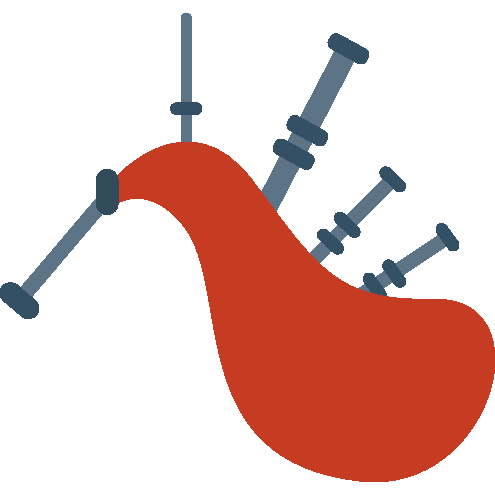
\includegraphics[scale=0.25]{bagpipes}};
\end{scope}


\end{tikzpicture}\newpage}

\foreach \x in {1,2,...,\loopmax}{%
\begin{tikzpicture}[xscale=-1,transform shape]
\path[use as bounding box] (0,0) rectangle (\textwidth,\textheight);

% 1. duck
\begin{scope}[xshift=\fpeval{1-\x*(1/\loopmax)}cm,yshift=0.1cm,scale=1.2]

\duck[body=DarkGoldenrod1!20!AntiqueWhite1,beret]
\begin{scope}
\path[clip]
\duckpathjacket;

\node[anchor=south west] at (0,0){
\includegraphics[width=3cm]{tartan3}};
\end{scope}
\draw[thick] \duckpathjacket;

\begin{scope}[rotate=-25]
\draw[line width=1.5pt] (0.13,2.15) ellipse (0.5 and 0.17)
            (0.13,2.25) ellipse (0.55 and 0.17)
	        (0.13,2.4) circle (0.08);
\end{scope}


\begin{scope}[rotate=-25]
\path[clip] (0.13,2.15) ellipse (0.5 and 0.17)
            (0.13,2.25) ellipse (0.55 and 0.17)
	        (0.13,2.4) circle (0.08);
\node[anchor=south west] at (-1,1){
\includegraphics[width=3cm]{tartan3}};
\end{scope}

\node[anchor=south west] at (-0.2,-0.55) {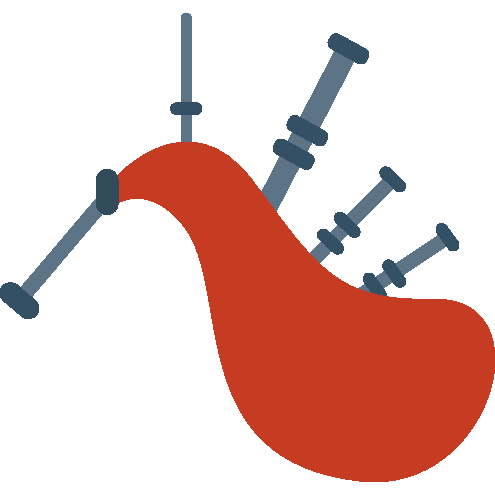
\includegraphics[scale=0.2]{bagpipes}};
\end{scope}

% 2. duck
\begin{scope}[xshift=\fpeval{5-\x*(1/\loopmax)}cm,yshift=0.1cm,scale=1.2]
\duck[body=DarkGoldenrod1!20!AntiqueWhite1,beret]

\begin{scope}
\path[clip]
\duckpathjacket;

\node[anchor=south west] at (0,0){
\includegraphics[width=3cm]{tartan3}};
\end{scope}
\draw[thick] \duckpathjacket;

\begin{scope}[rotate=-25]
\draw[line width=1.5pt] (0.13,2.15) ellipse (0.5 and 0.17)
            (0.13,2.25) ellipse (0.55 and 0.17)
	        (0.13,2.4) circle (0.08);
\end{scope}

\begin{scope}[rotate=-25]
\path[clip] (0.13,2.15) ellipse (0.5 and 0.17)
            (0.13,2.25) ellipse (0.55 and 0.17)
	        (0.13,2.4) circle (0.08);
\node[anchor=south west] at (-1,1){
\includegraphics[width=3cm]{tartan3}};
\end{scope}


\node[anchor=south west] at (-0.2,-0.55) {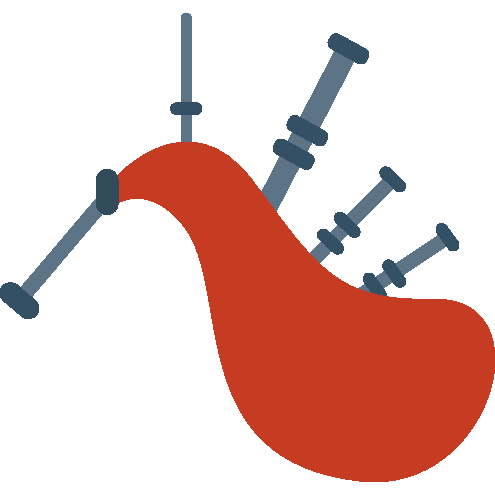
\includegraphics[scale=0.2]{bagpipes}};
\end{scope}

%3. duck
\begin{scope}[xshift=\fpeval{9-\x*(1/\loopmax)}cm,yshift=0.1cm,scale=1.2]
\duck[body=DarkGoldenrod1!20!AntiqueWhite1,beret]

\begin{scope}
\path[clip]
\duckpathjacket;

\node[anchor=south west] at (0,0){
\includegraphics[width=3cm]{tartan3}};
\end{scope}
\draw[thick] \duckpathjacket;

\begin{scope}[rotate=-25]
\draw[line width=1.5pt] (0.13,2.15) ellipse (0.5 and 0.17)
            (0.13,2.25) ellipse (0.55 and 0.17)
	        (0.13,2.4) circle (0.08);
\end{scope}


\begin{scope}[rotate=-25]
\path[clip] (0.13,2.15) ellipse (0.5 and 0.17)
            (0.13,2.25) ellipse (0.55 and 0.17)
	        (0.13,2.4) circle (0.08);
\node[anchor=south west] at (-1,1){
\includegraphics[width=3cm]{tartan3}};
\end{scope}


\node[anchor=south west] at (-0.2,-0.55) {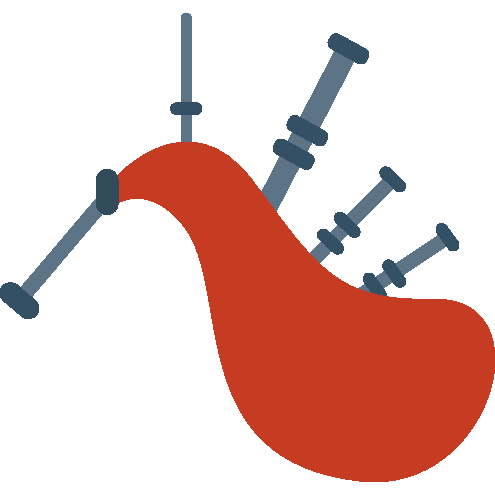
\includegraphics[scale=0.2]{bagpipes}};
\end{scope}


\end{tikzpicture}\newpage}

\end{document} 